% \chapter{Introduction}
\chapter{Field-Effect Penetration through Two-Dimensional Materials}
\label{ch:qc} \renewcommand*\imgdir{img/qc/}

% \dictum[H. C. Andersen \textit{The Emperor's New Clothes}]{%
  % ``But he has nothing on at all!'' said a little child at last.  }%


\vspace{1em}

\chapterabstract{This chapter is adapted from the following journal
article: Tian, T., Rice, P., Santos, E. J. G. \& Shih,
C.-J. Multiscale Analysis for Field-Effect Penetration through
Two-Dimensional Materials. Nano Lett. 16, 5044–5052 (2016).}


\newcommand*\subs[1]{_{\text{#1}}} % Text subscription, not available
for comma separated \newcommand*\sups[1]{^{\text{#1}}} %Text
superscription % \newcommand*\change[1]{\textcolor{cyan}{#1}}
\newcommand*\change[1]{}




\section{Introduction}
\label{sec:qc-introduction}

In this chapter, we study the question concerning the penetration of
electrostatic field effect through a 2D material, as we pointed in
\autoref{sec:electr-inter-thro}.
%
The field effect refers to the modulation of the space charge
concentration in a semiconductor by applying an electric displacement
field \autocite{Sze_2006_Mosfets}.  Over the past few decades, it has been
utilized to enable a wide range of electronics with
metal-oxide-semiconductor (MOS) architecture, including the
field-effect transistors (FETs) and the floating-gate memory devices
\autocite{Sze_2006_Mosfets}.
%
On the other hand, the two-terminal active electronic components, such
as diodes, which consist of semiconductor layers sandwiched between
two metallic electrodes, fundamentally prohibit introduction of the
field effect due to strong electric-field screening in metal
\autocite{Ehrenreich_2001_solidstate_phys}.
%
A possible workaround to induce the field effect through a conducting
electrode, is the concept of ``quantum capacitors
(QCs)''~\autocite{Luryi_1988_Quantum}.  In the original theoretical paper
by Luryi, a two-dimensional electron gas (2DEG) is used as one
terminal, allowing partial penetration of the field effect
\autocite{Luryi_1988_Quantum}.
%
The 2DEG was subsequently realized in the 1980s--1990s by trapping
electrons in a quantum well \autocite{Davies_1997_book,Ihn_2009_book} or
confining an inversion layer in a metal-oxide-semiconductor (MOS)
capacitor\autocite{Sze_2006_Mosfets}.
%
However, despite great success in demonstration of concept, there are
still several limitations: (i) the fabrication of 2DEGs typically
involves cumbersome molecular beam epitaxy (MBE) of
semiconductors~\autocite{Chang_2012_MBE}, (ii) the fabrication of 2DEG in
semiconductor heterostructures is limited to a few semiconductor
families due to the requirement of lattice matching (see
\autoref{sec:intro-3D-2D},~\autocite{Stormer_1979_2DEG}, and (iii) despite
the confinement of the quantum well, the 2DEG still spreads over a
distance of several nano\-meters, making it not strictly
two-dimensional~\autocite{Ihn_2009_book}.
%

Recent development in 2D material systems as discussed in
\autoref{sec:categ-2d-mater}, has further suggested new opportunities
in integrating them into different materials systems.
%
Due to the atomically thin feature of these materials, they have been
considered the ideal candidates of 2DEG
\autocite{Novoselov_2012_roadmap} to realize the QC devices on a large
scale.
%
In the past years, the idea of using graphene 2DEG as one terminal to
modulate the characteristics of the two-terminal electronic device via
gating has been utilized in many graphene-based vertical electronics
and vdW heterostructures
\autocite{Geim_2013_2D_vdw_Het,Novoselov_2016_vdW}, including vertical
transistors / barristors \autocite{Yang_2012_Barristor, Yu_2013_vertical,
georgiou2013vertical, Shih_2015_PartiallyScreened}, solar cells
\autocite{Yu_2013_gate_photocurrent, Britnell_2013_vdWE,
Regan_2012_ScreeningEngineered_PV} and light emitting diodes
\autocite{Withers_2015_LED_vde_Het}.
%
Indeed, most of these devices can be categorized as QCs at some
extension.
%
As briefly mentioned in \autoref{sec:electr-inter-thro}, the majority
of reports have attributed the observed gate-tunable transport
behavior to the change of graphene's work function, while the
penetration of the field effect through graphene 2DEG, as well as the
effect of the diode bias, are often ignored or over-simplified.
%
A more complete theoretical picture and analysis are required to
elucidate the graphene-based QCs in terms of the interplay between the
penetration of field effect and the electronic structure of the 2D
materials.

This chapter aims to present a multiscale theoretical approach to model
the space charge distribution in a metal-oxide-graphene-semiconductor
(MOGS) QC, giving a quantitative interpretation of the field-effect
penetration into the device.
%
We use both macroscopic modeling using Poisson-Boltzmann equation
methods and first-principles calculations at different levels of
accuracy to prove that the space charge density in the semiconductor
layer can be modulated by the field effect through the graphene 2DEG,
thereby creating an accumulation or inversion layer at the
graphene-semiconductor interface.
%
Accordingly, we define a field-effect ``transparency'' index
$\eta^{\mathrm{FE}}$ to quantify the penetration of an electric
displacement field through a 2DEG.
%
Using fundamental analysis, we show that $\eta^{\mathrm{FE}}$ is a
combined effect of the 2DEG quantum capacitance $C_{\mathrm{Q}}$, and
the semiconductor capacitance, $C\subs{S}$.
%
By combining with the density functional theory (DFT) calculations, we
have used the obtained analytical relations to rank a variety of 2D
(e.g. silicene, germanene, phosphorene and TMDCs) materials according
to their transparency to an electric displacement field.
%
Finally, the effect of the bias voltage applied on the semiconductor
terminal, $V\subs{b}$ is discussed.  Our analysis show that because
the semiconductor capacitance $C_{\mathrm{S}}$ increases significantly
with $V\subs{b}$, the penetration of the field effect in a MOGS QC
becomes much less effective beyond a certain $V\subs{b}$ range which
can guide to optimum design functioning rules.


\section{Results and Discussions}
\label{sec:qc-results-discussions-}

\subsection{Mean-Field Model Based on Poisson-Boltzmann Equation}
\label{sec:qc-mean-field-model}

In this section, a mean-field model based on the Poisson-Boltzmann
equation is derived to quantify the charge density distribution in a
MOGS QC.  \autoref{fig:qc-Scheme}\lc{a} shows a one-dimensional MOGS
system comprised of a metal (M) electrode, a dielectric oxide (O)
layer, a sheet of undoped monolayer graphene (G), and a bulk
semiconductor (S) layer with the thickness $d\subs{S}$
($d_{\mathrm{S}}$ is much larger than the Debye length in the
semiconductor).  A gate voltage $V\subs{M}$ is applied between the
metal and graphene terminals to electrostatically induce space charges
in graphene and the semiconductor layers.
%
An Ohmic contact is used on the semiconductor side to apply a bias
voltage $V\subs{b}$ between the semiconductor and graphene terminals.

\begin{figure}[!htbp] %
  \centering{}
  \import{\imgdir}{device.pdf_tex} %
  \caption{  The quantum capacitor based on 2DEG. \textbf{a}. Schematic illustration for the setup of a MOGS QC.  \textbf{b}.
Schematic band diagram of a MOGS QC.}
  \label{fig:qc-Scheme}
\end{figure}

First, the electroneutrality of the entire system suggests:
\begin{equation} \sigma\subs{M}+\sigma\subs{G}+\sigma\subs{S}=0
    \label{eqn:qc-charge-balance}
\end{equation} where $\sigma\subs{M}$ and $\sigma\subs{G}$ and
$\sigma\subs{S}$ are the surface charge densities in the metal,
graphene, and semiconductor terminals, respectively.  The $x$
coordinate is defined as the distance away from the
semiconductor/graphene (SG) interface in the semiconductor layer (see
\autoref{fig:qc-Scheme}\lc{b}). According to the Gauss's law,
$\sigma\subs{S}$ is given by:
\begin{equation} \sigma\subs{S} = \int_{0}^{d_{\mathrm{S}}}
\rho_{\mathrm{S}}(x) dx = -\varepsilon_{0}\varepsilon\subs{S}
\mathscr{E}_0
    \label{eqn:qc-sigma_S}
\end{equation} where $\rho_{\mathrm{S}}(x)$ is the space charge
density at position $x$ in semiconductor; $\varepsilon\subs{S}$ is the
relative permittivity of semiconductor, $\varepsilon_{0}$ is the
vacuum permittivity and $\mathscr{E}_0$ is the electric field at the
SG interface.
%
We assume that the electric potential in the semiconductor layer,
$\psi(x)$, satisfies the Poisson-Boltzmann
equation~\autocite{Sze_2006_Mosfets}:
\begin{equation}
    \label{eqn:qc-2nd-poisson} \frac{d^2 \psi(x)}{dx^2} =
-\frac{e\rho(x)}{\varepsilon_{0}\varepsilon_{\mathrm{S}}} = -
\frac{e}{\varepsilon_{0}\varepsilon\subs{S}}[p_0(\text{e}^{-\beta
\psi(x)}-1) - n_0(\text{e}^{\beta \psi(x)} -1)]
\end{equation} where $e$ is the elementary charge, $\beta=e/k\subs{B}
T$, $k\subs{B}$ is the Boltzmann constant, $T$ is temperature and
$n_0$, $p_0$ are the equilibrium electron and hole densities in bulk
semiconductor, respectively.
%
Considering the limit that the Debye length (see
\autoref{eq:intro-debye}) in the semiconductor layer
$\lambda_D\approx\sqrt{\dfrac{\varepsilon_{0} \varepsilon\subs{S}
k\subs{B} T}{e^2 N\subs{D}}}$ (where $N\subs{D}$ is the dopant
density) is much smaller than $d_{\mathrm{S}}$, the boundary
conditions $\psi(x=0)=\psi_0$, $\psi(\infty)=0$ and $\psi'(\infty)=0$
are used for \autoref{eqn:qc-2nd-poisson}, where $\psi_0$ is the
electric potential at the SG interface.
%
By integrating \autoref{eqn:qc-2nd-poisson} with respect to $x$, one
can determine the semiconductor space charge density $\sigma\subs{S}$
as a function of $\psi_0$ as follows:
\begin{equation}
    %%%%
    % Can be split into lines if using double column
    %%%%
    \label{eqn:qc-sigma_S_exact}
    \begin{aligned} \sigma\subs{S}(\psi_0) = &-\varepsilon\subs{S}
\mathrm{sign}(\psi_0)\sqrt{\frac{2e}{\beta \varepsilon\subs{S}}}\\
&\sqrt{p_0(\text{e}^{-\beta\psi_0} + \beta \psi_0 -1) +
n_0(\text{e}^{\beta\psi_0} - \beta \psi_0 -1) }
    \end{aligned}
\end{equation} where $\mathrm{sign}$ is the sign function.  The
electric potential at the SG interface, $\psi_0$ is determined by the
Schottky-Mott rule~\autocite{Sze_1965_defect}, which assumes that the
vacuum level alignment at the SG interface.
%
Note that this assumption holds when the interface states at the SG
interface are negligible
\autocite{Xu_2011_Inducing_charge_si,Hill_1998_Molecular_align}, which is
fulfilled due to the absence of dangling bonds on the graphene
surface.  We only consider inorganic semiconductor for this model,
since for the interface between graphene and organic semiconductor the
assumption of the vacuum level alignment does not hold
\autocite{Hill_1998_Molecular_align}.  The boundary condition imposed by the
Schottky-Mott rule~\autocite{Sze_1965_defect} follows that:
\begin{equation}
  \label{eqn:qc-Shottky-Mott} \psi_0 = \frac{E_{\mathrm C,\infty} -
E_{\mathrm F,\infty}}{e} - \phi\subs{G} + \chi\subs{S} - V\subs{b}
\end{equation} where $E_{\mathrm C,\infty}$ and $E_{\mathrm F,\infty}$
are the conduction-band (CB) and Fermi levels in semiconductor at the
flat-band condition, respectively, and $\chi\subs{S}$ is the electron
affinity of the semiconductor (see \autoref{fig:qc-Scheme}\lc{b}).
%
$\phi\subs{G}$ is the work function of graphene as a function of
$\sigma\subs{G}$, which is assumed to follow the elementary electronic
properties of graphene \autocite{Xu_2011_Inducing_charge_si} at 0 K,
without considering the electron-hole puddles induced by the
surroundings \autocite{Das_Sarma_2011_electron_gr}:
\begin{equation}
  \label{eqn:qc-phi-gr} \phi\subs{G} = \phi\subs{G}^{0} +
\mathrm{sign}(\sigma\subs{G})\frac{\hbar v\subs{F}}{e}\sqrt{\frac{\pi
|\sigma\subs{G}|}{e}}
\end{equation} where $\hbar$ is the reduced Planck constant,
$v\subs{F} \approx 1.1\times10^6 $ m$\cdot$s$\sups{-1}$ is the Fermi
velocity in graphene and $\phi^0\subs{G} = 4.6$ V is the work function
of graphene at the charge neutrality point (CNP, center of the Dirac
cone) corresponding to $\sigma\subs{G} = 0$ \autocite{Yu_2009_Tuning}.
%

An important feature of the 2DEG is its Fermi level $E_{\mathrm{F}}$
(or equivalent the work function $\phi$) depends on the charge density
$\sigma$, as a consequence of limited density of states (DOS, see
\autoref{sec:basic-electr-prop}) and Pauli's exclusion
principle.~\autocite{Luryi_1988_Quantum} The ability to change the Fermi
level of a 2DEG is characterized by its quantum capacitance
$C_{\mathrm{Q}}$. For graphene, $C_{\mathrm{Q}}$ is defined as:
\begin{equation}
  \label{eq:qc-def-qc} C_{\mathrm{Q}} = \frac{\partial
\sigma\subs{G}}{\partial \phi\subs{G}}
\end{equation} Due to a nonzero $C_{\mathrm{Q}}$ of graphene, the
application of $V\subs{M}$ to the MOGS QC considered here (
\autoref{fig:qc-Scheme}\lc{a}) includes the shift in the work function of
graphene, or namely,
\begin{align}
    \label{eqn:qc-V_M} V\subs{M} = \frac{\sigma_{M}}{C\subs{ox}} +
\int_{\sigma\subs{G}|_{V\subs{M}=0}}^{\sigma\subs{G}}
\frac{1}{C\subs{G}} d\sigma\subs{G}
\end{align} where $C\subs{ox}$ is the geometric capacitance of the
dielectric oxide layer defined as $C_{\mathrm{ox}} = \varepsilon_{0}
\varepsilon_{\mathrm{ox}} / d_{\mathrm{ox}}$, where
$\varepsilon_{\mathrm{ox}}$ is the permittivity of the oxide layer and
$d_{\mathrm{ox}}$ is the thickness of the oxide layer.
%
\autoref{eqn:qc-V_M} suggests that at $V\subs{M}$ = 0, $\phi\subs{G}$
does not necessarily coincide with the CNP, and depends on the doping
level of the adjacent semiconductor layer.
%
By combining \autoref{eqn:qc-charge-balance} and
\autoref{eqn:qc-sigma_S_exact}--\autoref{eqn:qc-phi-gr}, the electric
potential at the SG interface, $\psi_0$, as a function of
$\sigma\subs{M}$, can be determined analytically.
%
Subsequently, by using the boundary conditions $\psi(0)=\psi_0$ and
$\psi_0 = \sigma\subs{S}/(\varepsilon_{0}\varepsilon\subs{S})$ in
\autoref{eqn:qc-2nd-poisson}, the $\psi(x)$ profile is solved
numerically, allowing us to construct the associated band diagrams.

\subsection{Charge Distribution at the Graphene--Semiconductor
Interface}
\label{sec:qc-charge-distr-sg}

% \todo{Self check onwards} To model the charge distribution1 at the
SG interface, we consider a doped silicon (Si) layer in the MOGS QC
structure at $T=300$  K.
%
The parameters of Si are $\chi\subs{S} = 4.0$ V, the bandgap
$E\subs{g} = 1.12$ eV, $\varepsilon_{\mathrm{S}} = 11.8$ and the
intrinsic carrier concentration $n\subs{i} = 9.7\times10^9$ cm$^{-3}$
\autocite{Sproul_1991_si_carrier_conc}.
%
First we analyze the case of free contact between the graphene and the
semiconductor layers, \ie $\sigma\subs{G}+\sigma\subs{S}=0$ and
$V\subs{M}=V\subs{b}=0$.  \autoref{fig:qc-fermi-level-change}\lc{a}
presents the change of Fermi level in graphene, $\Delta E_{\mathrm
{F,G}} = -(\phi\subs{G} - \phi\subs{G}^0)$, as a function of the
equilibrium electron concentration $n_0$.
%
Note that when $n_0 < n\subs{i}$, the majority carriers are holes, \ie
the semiconductor is p-doped and \textit{vice versa}.
%
Indeed, in order to fulfill the Schottky-Mott rule, the work function
difference across the SG interface results in a charge transfer at the
interface.
%
A nearly symmetric response of $\Delta E_{\mathrm {F,G}}$ with respect
to the Si doping level reflects the fact that the intrinsic work
function, $\phi\subs{S}^0=4.56$ V, is very close to $\phi\subs{G}^0$.
%
When the Si layer is heavily doped ($>10^{15}$ cm$^{−3}$ for the
majority carrier), a relatively pronounced transfer of majority
carrier occurs, with a $\Delta E_{\mathrm {F,G}}$ up to $\pm$0.2 eV.

\begin{figure}[!htbp] %
    \centering{}
  \import{\imgdir}{EFermi-prof.pgf}
  \caption{ Fermi level and interfacial charge modulation in a MOGS
    QC.  \textbf{a}. The calculated Fermi level change of graphene,
    $\Delta E_{\mathrm {F,G}}$, as a function of $n_0$ in Si when
    considering free contact between the graphene and Si layers.
    \textbf{b}. The calculated $\Delta E_{\mathrm {F,G}}$ as a
    function of $\sigma\subs{M}$ in a MOG capacitor and a MOGS QC. The
    doping level of majority carrier in p-type/n-type Si is
    10$\sups{18}$ cm$\sups{-3}$.  \textbf{c}. The calculated $\psi_0$
    as a function of $\sigma\subs{M}$ in n-type ($N\subs{D}=10^{16}$
    cm$\sups{-3}$) MOS and MOGS capacitors. The accumulation (light
    blue) and strong inversion (pink) regimes are also shown for
    comparison.  (d) The calculated contour map of $\psi_0$ as a
    function of $\sigma\subs{M}$ and $n_0$. The accumulation (Ac),
    depletion (Dp), weak inversion (WI), and strong inversion (SI)
    regimes are labeled accordingly.  }
  \label{fig:qc-fermi-level-change}
\end{figure}

Next, we apply a nonzero $\sigma\subs{M}$ to the metal terminal,
corresponding to a $V\subs{M}$ described by \autoref{eqn:qc-V_M}.
%
A proper range of $\sigma\subs{M}$ up to $\pm$2$\times$10$^{13}$
$e\cdot$cm$^{-2}$, which can be reached by using a high-k dielectric
oxide layer
\autocite{Das_Sarma_2011_electron_gr,Schwierz_2010_Graphene_transistor}.
$\sigma\subs{M}$ and $\sigma\subs{S}$ are subsequently altered as a
result of the field effect.
%
The $\Delta E_{\mathrm {F,G}}$ -
$\sigma\subs{M}$ curves at different Si doping levels are shown in
\autoref{fig:qc-fermi-level-change}\lc{b}.  By solving
\autoref{eqn:qc-phi-gr} at $\sigma\subs{G}$ + $\sigma\subs{M}$ = 0,
the curve associated with a MOG QC is also shown for comparison.
%
As well-stated in literature
\autocite{Neto_2009_Electron_gr_rev,Das_Sarma_2011_electron_gr}, due to a
small DOS near the CNP of graphene,
$\Delta E_{\mathrm {F,G}}$ changes rapidly as $\sigma\subs{M}\to0$ in
the MOG QC.
%
In the range of $\sigma\subs{M}$ considered, one can tune
the Fermi level of graphene up to $\pm$0.5 eV.
%
On the other hand,
regarding the MOGS QCs in which graphene is in contact with a Si
layer, when an intrinsic silicon is used, we do not find a notable
difference until a relatively high $|\sigma\subs{M}|$ is applied.
%
Nevertheless, when the Si layer is heavily doped (either n- or
p-doping, with a majority dopant concentration of 10$^{18}$
cm$^{-3}$), a considerable deviation from the
$\Delta E_{\mathrm {F,G}}$ - $\sigma\subs{M}$ curve of MOG is
observed.
%
It suggests that $\sigma\subs{G}$+$\sigma\subs{M}$ (numerically
equivalent to -$\sigma\subs{S}$) becomes nonzero, or in other words,
the induced charges in graphene partially ``leak'' to the adjacent
semiconductor layer.
%
We therefore suggest that the estimation of graphene's work function
using $\phi\subs{G}|_{\sigma\subs{G}=-\sigma\subs{M}}$ in a MOGS QC,
as has been widely used to estimate the work function of graphene in a
MOGS QC (e.g. \autocite{Georgiou_2012_VFET_2D_vdw,georgiou2013vertical})
appears to be incorrect.
%
Indeed, in a MOGS QC, graphene behaves like
a 2DEG and is not capable of completely screening the electric
displacement field applied.

In order to further understand the penetration of the field effect
through graphene,
% \worktodo{change figure name}
\autoref{fig:qc-fermi-level-change}\lc{c} compares the
change of calculated $\psi_0$ with $\sigma\subs{M}$ in a standard
metal-oxide-semiconductor (MOS) capacitor and a MOGS QC ($N\subs{D}$ =
10$\sups{16}$ cm$\sups{-3}$), as a function of $\sigma\subs{M}$.
%
In a standard MOS capacitor, the field effect allows significant
modulation of the space charge concentration at the oxide-semiconductor
interface by applying a relatively small $\sigma\subs{M}$, such that
$\psi_{0}$ changes rapidly and moves beyond the conduction and valence
band (VB) energy levels ($E\subs{C}$ and $E\subs{V}$, respectively).
%
On the other hand, in a MOGS QC, the modulation of $\psi_0$ is
observed to be less sensitive to $\sigma\subs{M}$, suggesting that the
field effect only partially penetrates through
graphene~\autocite{Shih_2015_PartiallyScreened}.
%
Nevertheless, one can still tune $\psi_0$ from the strong inversion
(SI) regime (pink, corresponding to $p(x = 0) > N\subs{D}$) to the
accumulation (Ac) regime (light blue, corresponding to
$n(x = 0) > N\subs{D}$), but not to the band edges.
%
Clearly, unlike
the standard MOS capacitors, we predict that the MOGS QC devices
inherently do not facilitate fast switching by the field effect.

Another important observation in \autoref{fig:qc-fermi-level-change}\lc{b}
is that $\sigma\subs{G}$ also depends on the doping level of the
adjacent Si layer.
%
In order to further discuss this effect,
\autoref{fig:qc-fermi-level-change}d presents the contour map of
$\psi_0$ as functions of $\sigma\subs{M}$ and $n_0$.
%
We also
include three curves associated with: (i) $\psi_0=0$, (ii)
$\psi_0= -( E_{\mathrm F,\infty} - E_{\mathrm i,\infty})/e$, and (iii)
$\psi_0 = -2(E_{\mathrm F,\infty} - E_{\mathrm i,\infty})/e$, where
$E_{\mathrm i,\infty}$ is the intrinsic energy level of Si
at the flat-band condition.
%
Note that the three curves intersect at point
$(n\subs{i}$, $\sigma\subs{M}^0)$, where $\sigma\subs{M}^0$ is
given by
\begin{equation}
  \sigma\subs{M}^0 =
\mathrm{sign}(\phi\subs{G}^0-\phi\subs{S}^0)\frac{(\phi\subs{G}^0-\phi\subs{S}^0)^2
e^3}{\pi \hbar^2 v\subs{F}^2}
\end{equation}
Here $\phi\subs{S}^0$ is the work function of intrinsic
Si.
%
Following the convention in semiconductor physics
\autocite{Sze_2006_Mosfets}, the three curves divide the contour map into
four regimes as follows: (i) the accumulation (Ac), (ii) the depletion
(Dp), (iii) the weak inversion (WI), and (iv) the strong inversion
(SI).
%
As shown, within the $\sigma\subs{M}$ range considered, the
partially-penetrated field effect allows the induction of an inversion
or accumulation layer at the SG interface, unless the semiconductor
doping level is relatively high (with a majority carrier
concentration $> 10^{18}$ cm$^{-3}$).
%
The wide tunability of interfacial charge distribution results
from the following two facts: (i) $\sigma\subs{S}^0$ is very close to
$\sigma\subs{G}^0$, and (ii) the bandgap of Si is comparable to the tunable
range of graphene's Fermi level.
%
Our findings explain why Si has been considered a good
semiconductor candidate in the MOGS QCs
\autocite{Yang_2012_Barristor,Schwierz_2010_Graphene_transistor,
  ,Regan_2012_ScreeningEngineered_PV}.


\subsection{The Field-Effect Transparency}
\label{sec:qc-field-effect-transp}

Based on the above analysis, we propose and derive an expression for
the field-effect transparency index $\eta^{\mathrm{FE}}$ that
quantifies the degree of penetration of an electric displacement
field in a MOGS QC as follows:
\begin{equation}
    \label{eqn:qc-def_eta}
  \eta^{\mathrm{FE}} = -\left(\frac{\partial
\sigma\subs{S}}{\partial \sigma\subs{M}}\right)
\end{equation}

%
Simply transforming \autoref{eqn:qc-def_eta} gives
$-(\partial \sigma\subs{G} / \partial
\sigma\subs{M})=1-\eta^{\mathrm{FE}}$, and by taking that (i)
$(\partial \phi\subs{G}/\partial \psi\subs{S})=-1$ (see
\autoref{eqn:qc-Shottky-Mott}) and (ii) the quantum capacitance of
graphene
$C_{\mathrm{Q}}=\partial \sigma\subs{G} / \partial \phi\subs{G}$ and
(iii) the differential capacitance of
semiconductor~\autocite{Sze_2006_Mosfets}
$C\subs{S} = -(\partial \sigma\subs{S}/ \partial \psi_0)$, the
transparency index $\eta^{\mathrm{FE}}$ in \autoref{eqn:qc-def_eta}
can be decomposed using the chain rule as:
\begin{equation}
  \begin{aligned}
  \label{eqn:qc-eta_expanded}
    \eta^{\mathrm{FE}} &= \left(\frac{\partial
\sigma\subs{S}}{\partial \psi_0}\right) \left(\frac{\partial
\sigma\subs{G}}{\partial \phi\subs{G}}\right)^{-1}
\left(\frac{\partial \sigma\subs{G}}{\partial \sigma\subs{M}}\right)\\
&= \frac{1}{1+C_{\mathrm{Q}}/C\subs{S}}= \left(1+\frac{2}{\hbar v\subs{F}}
\sqrt{\frac{e^3
|\sigma\subs{G}|}{\pi}}\frac{\mathscr{E}_0}{\rho_0}\right)^{-1}
\end{aligned}
\end{equation}
% 
where $\rho_0$ is the charge density at the SG
interface.

Accordingly, the contour plot of $\eta^{\mathrm{FE}}$ as a function of
$\sigma\subs{M}$ and $n_0$ is shown in
\autoref{fig:qc-transparency-MOGS}.
\begin{figure}[!htbp] %
    \centering{}
  \import{\imgdir}{eta-fe.pgf}
  \caption{Calculated transparency of graphene 2DEG to electric
    displacement field in a MOGS QC, as functions of $\sigma\subs{M}$
    and $n_0$. }
  \label{fig:qc-transparency-MOGS}
\end{figure}           
%
\autoref{eqn:qc-eta_expanded}
suggests that the transparency of graphene 2DEG to an electric
displacement field is determined by the combined effects of the
graphene quantum capacitance and the semiconductor capacitance.
%
As a result, the limit of perfect transparency,
$\eta^{\mathrm{FE}} \to 1$, would occur when $C_{\mathrm{Q}} \to 0$,
corresponding to the CNP of graphene, along the curve of $\psi_0=0$ in
\autoref{fig:qc-fermi-level-change}d.
%
However, we observe that such
transparency disappears by even slightly changing $\sigma\subs{M}$, due to
the rapid increase of $\phi\subs{G}$ with $\sigma\subs{G}$ near the
CNP of graphene.
%
In practice, considering the
residual charges induced by the electron-hole puddles near the CNP of
graphene \autocite{Das_Sarma_2011_electron_gr},
%
we expect that the limit of $\eta^{\mathrm{FE}} \to 1$ may not be
observable experimentally at room temperature.
%
On the other hand, a general trend exhibited in
\autoref{fig:qc-transparency-MOGS} is that one can gain a higher
degree of transparency for the graphene 2DEG by either (i) increasing
the doping level in the Si layer or (ii) applying a higher
$|\sigma\subs{M}|$, both resulting a considerable increase of
$C\subs{S}$.
%

Note in real experimental conditions, the interfacial states at the
semiconductor interface may also have influence on the field-effect
transparency. We consider a classical model that takes the interface
states as a thin layer of ionized species at the semiconductor
surface, with a distribution thickness of $d_{\mathrm{I}}$ and
effective permittivity of $\varepsilon_{\mathrm{I}}$
~\autocite{Heine1965_surface_theory,Sze_1965_defect}.
%
%
\begin{figure}[!htbp]
  \centering
  % 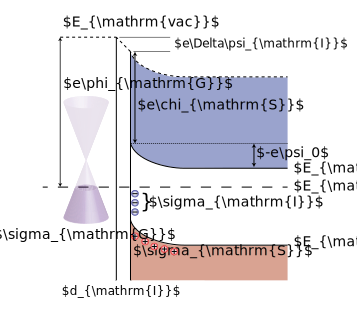
\includegraphics[width=0.65\textwidth]{img/scheme_interfacial.eps}
  \import{\imgdir}{scheme_interfacial.pdf_tex}
  \caption{Scheme for the graphene-semiconductor interface with interface states.}
  \label{fig:qc-scheme-interface}
\end{figure}
%
As schematically shown in \autoref{fig:qc-scheme-interface}, the
interface states possess a constant charge density of
$\sigma\subs{I}$, which create a potential drop
$\Delta \psi_{\mathrm{I}}$ over the interface layer.
%
% According to
% Gauss's law, $\Delta \psi_{\mathrm{I}}$ i:
% \begin{equation}
  % \Delta = d\subs{I}\frac{\sigma\subs{S}+\sigma\subs{I}}{\epsilon\subs{I}}
  % \label{eqn:delta_1}
% \end{equation}
The new boundary condition for energy level at the SG interface considering the interfacial states, is given by:
\begin{equation}
  \label{eqn:qc-shottkey-I}
  \Delta \psi_{\mathrm{I}} = \frac{E_{\mathrm C,\infty} - E_{\mathrm F,\infty}}{e} + \chi\subs{S} -\psi_0 - \phi\subs{G} = d\subs{I}\frac{\sigma\subs{S}+\sigma\subs{I}}{\epsilon\subs{I}}
\end{equation}
Similar to \autoref{eqn:qc-eta_expanded}, $\eta^{\mathrm{FE}}$ considering the effect of interfacial states, becomes:
\begin{equation}
  \begin{aligned}
    \label{eq:qc-eta-I-1}
      \eta^{\mathrm{FE}} 
           &= \dfrac{1}{1 - \dfrac{C\subs{Q}}{C\subs{S}}\dfrac{\partial \phi\subs{G}}{\partial \psi_0}}\\
           &= \dfrac{1}{1+k\dfrac{C_{\mathrm{Q}}}{C_{\mathrm{S}}}}
  \end{aligned}
\end{equation}
where
$k = -\left(\partial \phi_{\mathrm{G}} / \partial \psi_{0}\right)$.
%
Note without the interfacial states, \autoref{eqn:qc-Shottky-Mott}
indicates $k = 1$, and \autoref{eq:qc-eta-I-1} reduces to
\autoref{eqn:qc-eta_expanded}.
%
Combining \autoref{eqn:qc-Shottky-Mott} and
\autoref{eqn:qc-shottkey-I}, we finally obtain:
\begin{equation}
  \begin{aligned}
    \label{eq:qc-eta-I-final}
      \eta^{\mathrm{FE}} 
           &= \dfrac{1}{1+\dfrac{C\subs{Q}}{C\subs{I}} +\dfrac{C\subs{Q}}{C\subs{S}} }
  \end{aligned}
\end{equation}
where
$C\subs{I}=\dfrac{\varepsilon_{0}\varepsilon\subs{I}}{d\subs{I}}$ is
the effective geometric capacitance of the interfacial layer.
Accordingly, the field-effect transparency is reduced by the
additional term $\dfrac{C\subs{Q}}{C\subs{I}}$ compared with the ideal semiconductor surface ($d_{\mathrm{I}} \to 0$).
%
In practice, although the interface states are difficult to be removed
completely,
%
their influence can be minimized by creating a clean surface in vdW
heterostructures~\autocite{Withers_2015_LED_vde_Het}.
%
Thereafter, we still use the expression of
\autoref{eqn:qc-eta_expanded} to simplify the following analysis in
this chapter.
%
Nevertheless, more experimental techniques are required to gain better
insights at the 2D material-bulk semiconductor interface.


\subsection{Comparison with First Principle Simulations}
\label{sec:qc-comp-with-first}

The above analysis based on Poisson-Boltzmann equation is still valid
at different levels of theory as demonstrated by first principles
simulations within density functional theory (DFT) (see
\autoref{sec:qc-methods} for details).
%
\begin{figure}[!htbp] %
    \centering{}
  \import{\imgdir}{first_principles.pdf_tex}
% \includegraphics[width=0.95\linewidth]{img/FIG2.eps} %
% 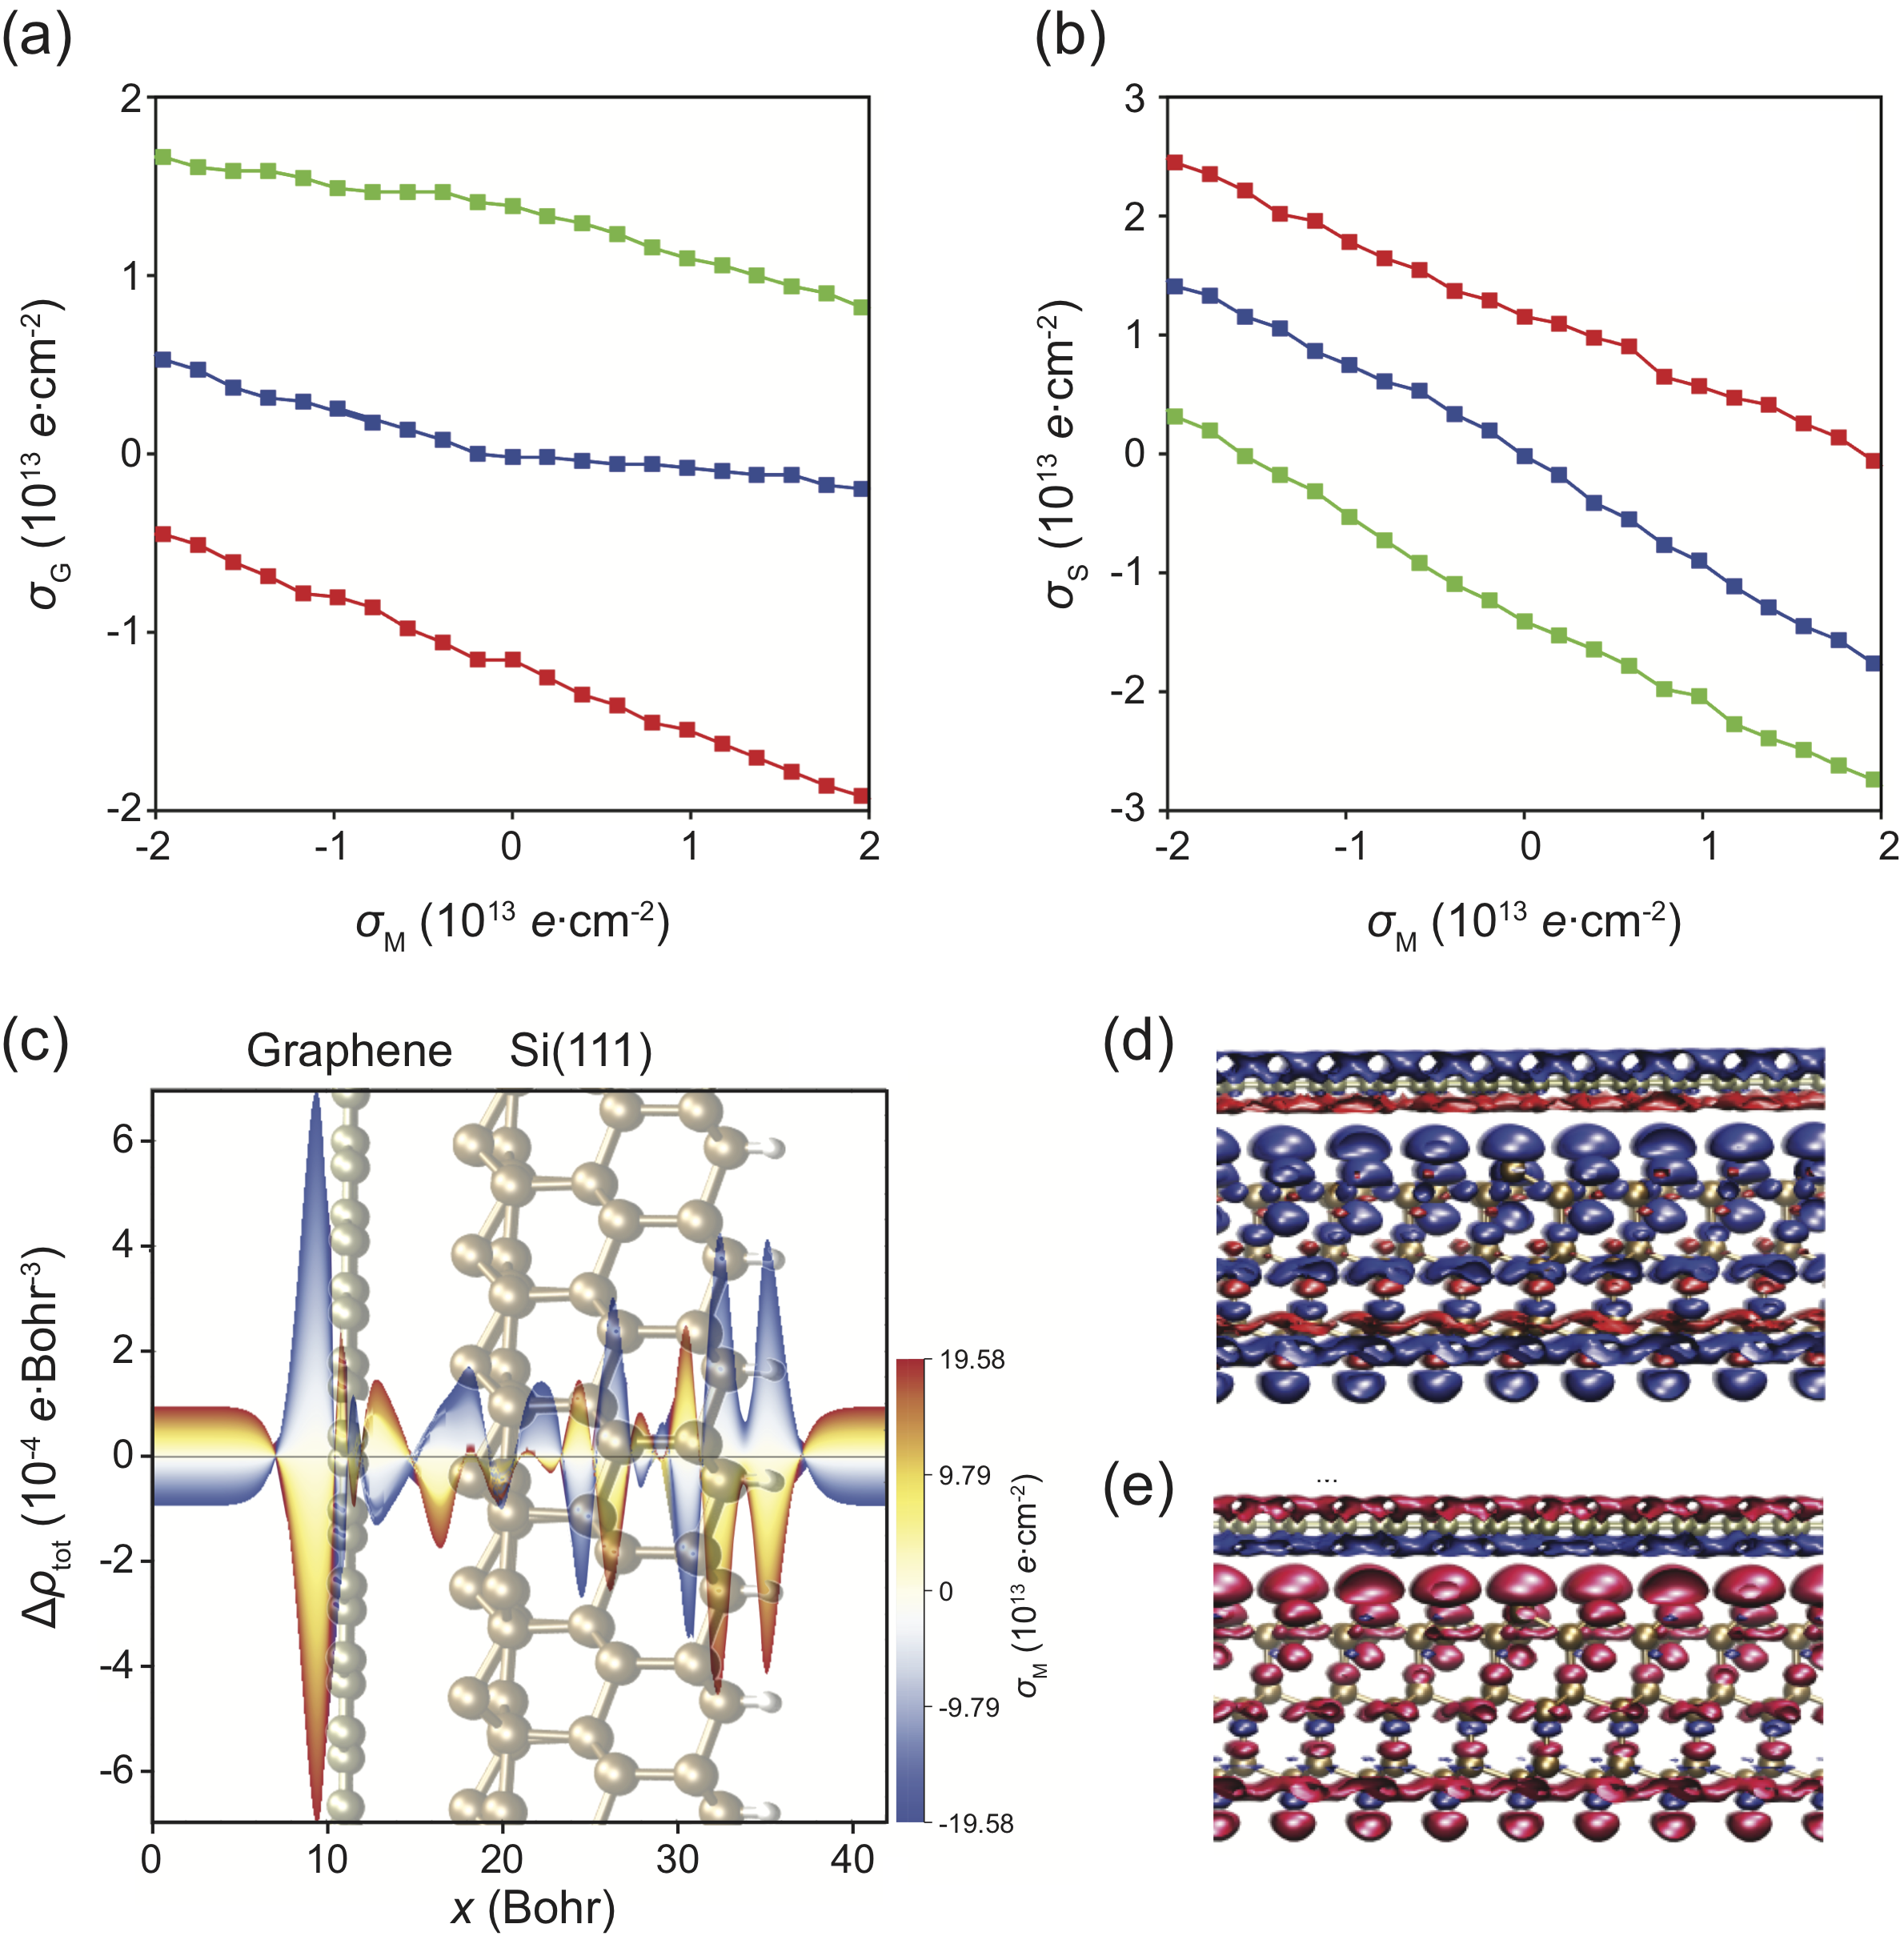
\includegraphics[width=0.95\linewidth]{img/FIG4.eps}
  \caption{
Field-effect transparency from first principles simulations.
    Induced charge densities at \textbf{a}. graphene, $\sigma\subs{G}$,
and \textbf{b}. Si(111), $\sigma\subs{S}$, as a function of $\sigma\subs{M}$
in different systems: intrinsic (blue), p-type (green) and n-type
(red) Si are plotted respectively.
%
The insets show the same data with smaller degree of metal charge $\sigma_{\mathrm{M}}$.
%
\textbf{c}. 3D
visualizations of the induced charge density contour in graphene and intrinsic
Si layers (cutoff at $\pm 2.1\times{}10^{-3}\ e\cdot$Bohr$^{-3}$) when 
$\sigma\subs{M}=-0.98\times10^{13}\ e\cdot$cm$\sups{-2}$ (top) and 
$\sigma\subs{M}=0.98\times10^{13}\ e\cdot$cm$\sups{-2}$ (bottom).  Blue and red
isosurfaces represent positive and negative charges, respectively.
%\protect \todo[inline]{Is the description for doping density right?}
  \label{fig:qc-first-principle}
}%
\end{figure}
%
\autoref{fig:qc-first-principle} shows the
calculated electronic response on a graphene\allowbreak{}/Si(111)
interface considering the effect of
gating.
%
We find that, irrespective of the doping levels considered, both
$\sigma\subs{G}$ and $\sigma\subs{S}$ monotonically decrease as
$\sigma\subs{M}$ increases (\autoref{fig:qc-first-principle}\lc{a}
and \lc{b}).
%
Similar to \autoref{fig:qc-fermi-level-change}\lc{b}, the amount of
induced charges in both graphene and Si layers as a result of
$\sigma\subs{M}$ depends on the doping density in the Si layer.
%
These results indicate that the field-effect transparency of the
graphene 2DEG is also valid at the quantum mechanical level.
%
We also observe that both $\sigma\subs{G}$ and $\sigma\subs{S}$ show a
nearly linear relation with $\sigma\subs{M}$ when very high
$\sigma\subs{M}$ (up to $\pm20\times10^{13}$ $e\cdot$cm$^{-2}$) is
applied.
%
This allows us to extract the
$\eta^{\mathrm{FE}}$ by performing a linear-regression to the
$\sigma\subs{S}-\sigma\subs{M}$ data using the formula
$\sigma\subs{S}=-\eta^{\mathrm{FE}} \sigma\subs{M} + b$, where $b$ is
a constant.
%
Interestingly, regardless of the Si doping level, all three systems
(intrinsic, p-doping and n-doping) show a $\eta^{\mathrm{FE}}$ $\sim{}$0.70.
%
These observations can be explained by \autoref{eqn:qc-eta_expanded}:
the few-layer Si used in the first principles simulations behaves more
like a 2D than bulk material, of which the quantum capacitance
$C\subs{S}$ remains almost constant when charges are filled into its
valence band (VB) or conduction band (CB) \autocite{Davies_1997_book}.
%
Conversely, when the doping level of graphene is extremely high, its
quantum capacitance $C_{\mathrm{Q}}$ will be less dependent of the
charge density after the van Hove singularity is reached
\autocite{Das_Sarma_2011_electron_gr}.
%
According to
\autoref{eqn:qc-eta_expanded},
$\eta^{\mathrm{FE}}=(1+C_{\mathrm{Q}}/C\subs{S})^{-1}$, if both
$C_{\mathrm{Q}}$ and $C\subs{S}$ are nearly constant, the
$\eta^{\mathrm{FE}}$ value becomes independent of either
$\sigma\subs{M}$ or Si doping level.
%
Moreover, since $C\subs{S}$ is
essentially larger than $C_{\mathrm{Q}}$ in this case as a result of
higher DOS of Si in the VB and CB, it is plausible to have a
$\eta^{\mathrm{FE}}$ larger than 0.5.
%

We also study the charge distribution over the SG interface as a
function of $\sigma\subs{M}$, which exhibits an intriguing profile as
shown in the electron density plots in
\autoref{fig:qc-first-principle}\lc{c} for a graphene layer and an
intrinsic Si slab.
%
The larger contours of the charge density at the SG interface
corresponds to the charge accumulation seen in \autoref{fig:qc-fermi-level-change}.
%
It is also found that that most of the orbitals that contribute to the
polarization of charge are the $2p\subs{z}$ in graphene and
$3p\subs{z}$ in Si, dependent on the polarity of $\sigma\subs{M}$
applied.
%
According to the results above, we find a
good consistency between the macroscopic model and first-principles
calculations, which allows us to perform a multiscale analysis for the
transparency of graphene 2DEG to an electric displacement field.
        

\subsection{General Behavior of 2DEG in Quantum Capacitor}
\label{sec:qc-gener-behav-2deg}

The intriguing  behavior at the SG interface draws our attention to
the possibility of replacing graphene in a MOGS QC structure with
other 2D materials.
%
% Indeed, as addressed earlier, the ultra-thinness
% of these materials suggests good potential for 2DEGs.
Under the
assumption that a 2D material-semiconductor interface satisfies the
Schottky-Mott rule, it is suggested that the relation of
$\eta^{\mathrm{FE}}=(1+C\subs{Q}/C\subs{S})^{-1}$ still holds.
%
Since the quantum capacitance is related with the DOS of 2D material by
$C\subs{Q} = \mathrm{DOS}(E) e^2$ \autocite{John_2004_QC},
%
we have calculated the DOS as a function of $E$ for a variety of 2D
materials\autocite{Xu_2011_Measure_QC_model, ,Jimenez_2012_drift_model_MoS2, ,Nawaz_2016_QC_silicene}
using the density functional theory (DFT) at the hybrid functional
level.
%
\begin{figure}[!htbp]
  \centering %
  \import{\imgdir}{QC_compare.pdf_tex}
% \includegraphics[width=0.95\textwidth]{img/FIG5.eps}
  \caption{Calculated quantum capacitances ($C\subs{Q}$) for the 2D
    materials considered, TMDs (MX$\subs{2}$, M = Mo, W; X = S, Se,
    Te), phosphorene, silicene, germanene and graphene, as a function
    of the \textbf{a}. electron density $\sigma\subs{2D}\sups{n}$ and
    \textbf{b}. hole density $\sigma\subs{2D}\sups{p}$.
    \textbf{c}. Geometries used to calculate the QC using HSE06
    hybrid functional for graphene, silicene/germanene, TMDCs and
    phosphorene.  The unit cell used in the simulations is highlighted
    in each panel.}
  \label{fig:qc-CQ-2D}
\end{figure} %
The relation between DOS and $C_{\mathrm{Q}}$ %
allows us to compare $\eta^{\mathrm{FE}}$ of a large variety of 2D
materials, including TMDC monolayers (MX$\subs{2}$, M = Mo, W; X = S,
Se, Te), silicene, germanene, and phosphorene.
%
The charge density in a 2D material is calculated by integrating the
DOS from its intrinsic Fermi level, \ie
$\sigma\subs{2D}=\int_{E\subs{F}}^{E} \mathrm{DOS}(E')e dE'$.
%
The calculated values of $C_{\mathrm{Q}}$ for the 2D materials
considered as a function of the electron or hole density are shown in
\autoref{fig:qc-CQ-2D}\lc{a} and \autoref{fig:qc-CQ-2D}\lc{b},
respectively.

As discussed in \autoref{sec:basic-electr-prop}, $C_{\mathrm{Q}}$ of a
monolayer 2D semiconductor  behaves
like a step function,
and only increases slightly with $\sigma\subs{2D}$, close to that for
an ideal 2D semiconductor with parabolic $E-k$ dispersion \autocite{Davies_1997_book}.
%
On the other hand, the quantum capacitance of a 2D semimetal,
including graphene, silicene, and germanene, exhibits a quadratic
relation with respect to $\sigma\subs{2D}$, because they share the
same feature of linear $E-k$ dispersion.
%
More importantly, the
quantum capacitance for the 2D semimetals are always less than those
for the 2D semiconductors under the same charge density. In other
words, although there are no states in the band gap, the DOS above the
band edge in a 2D semiconductor is significantly higher compared to
that in a semimetal, reflecting the fact that the effect mass of
carriers $m^{*}$ in the 2D semiconductors is much higher than that in the 2D
semimetals.
%
This concept also explains why the $C\subs{Q}$ for silicene and
germanene are similar but higher than that in graphene, in accordance
with other theoretical
investigations~\autocite{Yan_2013_e-hv-couple,Bechstedt_2012_silicene}.
Combining with \autoref{eqn:qc-eta_expanded}, the observations have
led to the conclusion that graphene exhibits the highest transparency
to an electric displacement field among all the 2D materials
considered here.
%
The theoretical framework also allows us to rank the 2D materials
according their transparency. For example, when the majority carrier
is electron, the following rank is predicted: graphene > silicene >
germanene > WS$\subs{2}$ > WTe$\subs{2}$ > WSe$\subs{2}$ >
MoS$\subs{2}$ > phosphorene > MoSe$\subs{2}$ > MoTe$\subs{2}$.
  % \change{ The above analysis for field-effect
  % transparency through multilayer graphene can also be applied to
  % other 2D materials.  Indeed, the total DOS of a multilayer 2D
  % material increases with layer number, leading to a higher
  % $C\subs{Q}$ and consequently lower field transparency.  }

Finally, we discuss the effect of the bias $V\subs{b}$ between the
semiconductor and graphene terminals. \autoref{eqn:qc-sigma_S_exact} and \autoref{eqn:qc-Shottky-Mott} have
suggested that a nonzero $V\subs{b}$ changes $\psi_0$ and
$\sigma\subs{S}$, and in order to satisfy the electroneutrality of the
system imposed by \autoref{eqn:qc-charge-balance}, an adjustment of
the $\phi\subs{G}$ occurs.
%
This behavior is different from the
semiconductor-metal (SM) interface.
%
Specifically, \autoref{fig:qc-chara-bias}\lc{a}
illustrates the main differences between SM and SG interfaces.
%
In an SM junction, the Schottky barrier height
$\varphi\subs{b}$ remains constant ($\varphi\subs{b}^0$) with respect to
$V\subs{b}$, because the work function of metal is independent of its
charge density.
%
As a result, the surface potential of the
semiconductor $\psi_{0}$ increases linearly with $V\subs{b}$.
%
On the contrary, in a semiconductor-graphene
(SG) junction, under a reverse bias with $V\subs{b}$ > 0, compare with the zero-bias case, one expect a more negative $\mathscr{E}_0$ followed by an increase in $\sigma\subs{S}$, and it is the other way
around for $V\subs{b}$ < 0.
%
As a result, 
$\sigma\subs{G}$ as well as the resulting $\psi_0$ and
$\phi\subs{b}$, exhibit a nonlinear dependence on $V\subs{b}$.
%
\begin{figure}[!htbp]
  \centering %
  \import{\imgdir}{bias-effect.pdf_tex}
  \caption{ The effect of $V\subs{b}$ in a MOGS QC. \textbf{a}. Schematic
illustration of the difference between a semiconductor-metal (SM) and
a semiconductor-graphene (SG) junction.  \textbf{b}. Calculated $\psi_0$ as a
function of $V\subs{b}$, under different $\sigma\subs{M}$ values. The
arrow indicates the direction of increasing $\sigma\subs{M}$.  \textbf{c}.
Calculated $\Delta E_{\mathrm{F,G}}$ as a function of $\sigma\subs{M}$
under different $V\subs{b}$ values. The arrow indicates the direction
of increasing $V\subs{b}$.  An n-type Si with $N\subs{D}=10^{16}$
cm$^{-3}$ is considered for \textbf{b} and \textbf{c}.  }
  \label{fig:qc-chara-bias}
\end{figure}

Taking a MOGS QC using an n-type Si (with donor concentration
$N\subs{D} = 10^{16}$ cm$^{-3}$) as an example, the calculated
$\psi_0$ as a function of $V\subs{b}$ under various $\sigma\subs{M}$
values applied is shown in \autoref{fig:qc-chara-bias}\lc{b}.
%
Compared with
the case of $V\subs{b} = 0$,
% in which a relatively wide range of
% $\psi_0$ can be tuned by $\sigma\subs{M}$, it is found that, by
% increasing $|V\subs{b}|$,
in both forward and reverse bias regimes 
$\psi_0$ becomes less tunable by $\sigma\subs{M}$.
%
In other words, $\sigma\subs{M}$ is losing control over the graphene's
Fermi level $E_{\mathrm {F,G}}$, when a higher $|V\subs{b}|$ is
applied.  We rationalize this observation by evaluating
$E_{\mathrm {F,G}}$ with respect to $\sigma\subs{M}$ under constant
$V\subs{b}$, or namely,
$(\partial E_{\mathrm {F,G}}/\partial \sigma\subs{M})_{V\subs{b}}$.
Combining the
relation $(\partial \phi\subs{G}/\partial \psi_0)_{V\subs{b}}=-1$ (see
\autoref{eqn:qc-Shottky-Mott}) with \autoref{eqn:qc-eta_expanded}, it
follows:
\begin{equation}
  \label{eqn:qc-tunability_gate}
  \begin{aligned}               %
    \left(\frac{\partial E_{\mathrm {F,G}}}{\partial
        \sigma\subs{M}}\right)_{V\subs{b}} &= -\left(\frac{\partial
        \phi\subs{G}}{\partial \sigma\subs{M}}\right)_{V\subs{b}} =
    \left(\frac{\partial \psi_0}{\partial
        \sigma\subs{S}}\right)_{V\subs{b}} \left(\frac{\partial
        \sigma\subs{S}}{\partial \sigma\subs{M}}\right)_{V\subs{b}}\\
    &= \frac{\eta^{\mathrm{FE}}}{C\subs{S}} =
    \frac{1}{C_{\mathrm{Q}}+C\subs{S}}= (\frac{2}{\hbar v\subs{F}}
    \sqrt{\frac{e^3 |\sigma\subs{G}|}{\pi}} +
    \frac{\rho_0}{\mathscr{E}_0})^{-1}
  \end{aligned}
\end{equation}                  %
Considering only a slight degree of band bending at
$|V\subs{b}|=0$, as shown in \autoref{fig:qc-chara-bias}\lc{a}, when a high
forward or reverse $|V\subs{b}|$ is applied, an inversion or
accumulation layer is formed at the SG interface.
%
The high degree of band bending in such conditions essentially
increases the capacitance of semiconductor $C\subs{S}$.
%
In order to
balance the induced $\sigma\subs{S}$, $\sigma\subs{G}$ also increases,
thereby yielding a higher $C_{\mathrm{Q}}$.
%
As suggested by
\autoref{eqn:qc-tunability_gate}, a simultaneous rise of $C\subs{S}$
and $C_{\mathrm{Q}}$ under a high $|V\subs{b}|$ results in a
significant decrease of
$(\partial E_{\mathrm {F,G}}/\partial \sigma\subs{M})_{V\subs{b}}$, or
the tunability of $E_{\mathrm {F,G}}$ with respect to
$\sigma\subs{M}$, as shown in \autoref{fig:qc-chara-bias}\lc{c}.
%
% Representative band diagrams of a MOGS QC are shown in Supporting
% Information S3.
This finding is consistent with the experimental
observations that the on/off current ratio is lowered by applying a
higher drain bias in a graphene-based vertical transistors
\autocite{Yang_2013_gr_hBN, ,Yu_2013_vertical, ,georgiou2013vertical,
  ,Shih_2015_PartiallyScreened, ,Schwierz_2010_Graphene_transistor}.
%
That is to say,
we suggest that the gate-tunable characteristics in a MOGS QC are only
observable in a certain $|V\subs{b}|$ range.  To our knowledge, this
effect has not been well discussed in literature.

\section{Conclusions}
\label{sec:qc-conclusions}

In this chapter, we have presented the multiscale approach to
understand the penetration of the field effect through a monolayer 2D
material in a metal-oxide-2D material-semiconductor quantum capacitor.
By using graphene as the model system, first we develop a macroscopic
model to describe the charge distribution in graphene and the
semiconductor layers by applying a $\sigma\subs{M}$ on the metal
electrode.  Depending on the degree of $\sigma\subs{M}$, the space
charge density in the semiconductor layer is modulated non-linearly,
forming an accumulation or inversion layer at the
semiconductor/graphene interface, which suggests that graphene is
partially ``transparent'' to an electric displacement field. These
results are corroborated by {\itshape ab initio} calculations at the
level of density functional theory including van der Waals
interactions.

We therefore define and formulate the degree of transparency of a
monolayer 2D material to an electric displacement field,
$\eta^{\mathrm{FE}}$, and show that $\eta^{\mathrm{FE}}$ is determined
by the combined effect of graphene quantum capacitance
$C_{\mathrm{Q}}$ and the differential capacitance of semiconductor
$C_{\mathrm{S}}$.
%
By calculating the quantum capacitance for a
variety of 2D materials using hybrid functional, we predict the
ranking for a variety of 2D compounds according to their transparency
to an electric displacement field as follows: graphene >
  silicene > germanene > WS$\subs{2}$ > WTe$\subs{2}$ > WSe$\subs{2}$
  > MoS$\subs{2}$ > phosphorene > MoSe$\subs{2}$ > MoTe$\subs{2}$,
when the majority carrier is electron.  Finally, the effect of the
voltage applied between the semiconductor and graphene terminals
$V\subs{b}$ is discussed.  Because a significant increase of the
semiconductor capacitance with $|V\subs{b}|$ in either reverse or
forward bias regime, we find that the gate-tunable characteristics in
a MOGS QC are only effective in a certain $|V\subs{b}|$ range, which
is often ignored in previous reports.  We believe that the development
of 2D materials-based quantum capacitors and vdW heterostructures will
be greatly facilitated by the fundamental principles and theoretical
analysis presented here.


\section{Methods}
\label{sec:qc-methods}

\subsection*{First Principles Simulations}
\label{sec:qc-first-princ-simul}

The first-principles simulations reported here are
based on density functional theory calculations using the {\ttfamily
SIESTA} method\autocite{Soler_02_siesta} and the {\ttfamily VASP}
code\autocite{Kresse_93_open_shell,Kresse_1996_1}.
%
The generalized gradient approximation(GGA)\autocite{Perdew_1996_GGA}
along with non-local van der Waals density functional for the
exchange-correlation term\autocite{Dion_2004_vdw} have been used.
%
A double-$\zeta$ polarized basis set in {\ttfamily SIESTA}, and a
well-converged plane-wave cutoff of 400 eV in {\ttfamily VASP} were
utilized in the calculations. Projected augmented wave method
(PAW)\autocite{Blochl_1994_PW,Kresse_1999_pseudopotentials} for the latter, and norm-conserving
Troullier-Martins pseudopotentials\autocite{troullier91} for the former,
have been used in the description of the bonding environment at the
different systems.  Atomic coordinates were allowed to relax until the
forces on the ions were less than 0.04 eV/\AA~under the conjugate
gradient algorithm.  Further relaxations (0.01 eV/\AA) do not change
appreciably the energetics and geometries.  To avoid any interactions
between supercells in the non-periodic direction, a 15 \AA~vacuum
space was used in all calculations. In addition to this, a cutoff
energy of 150 Ry was used to resolve the real-space grid used to
calculate the Hartree and exchange-correlation contribution to the
total energy.  A basis set of numerical atomic orbitals obtained from
the solution of the atomic pseudopotential at slightly excited states
as implemented in the {\ttfamily SIESTA}\autocite{Soler_02_siesta} code was
used. We have utilized an energy shift of 50 meV to define the radii
of different orbitals.  To model the Si surface, we used a periodic
array of 4-layer Si(111) slabs, separated by 15 \AA~ thick vacuum
space, and terminated by hydrogen atoms at the bottom.  Only the two
top layers were allowed to relax in contact with graphene, while the
rest were kept frozen at Si bulk lattice constant.  We have also
carried out calculations using screened hybrid functional at the
level of Heyd-Scuseria-Ernzerhof (HSE06) approach\autocite{Heyd_2003_HSe,HSE_2006_erratum}. In this
approximation part of the short range exchange energy is replaced by a
portion of exact Hartree-Fock exchange energy.  Here we used HSE06 as
an example of a hybrid functional because of its successful
applications in solids and
molecules\autocite{Kresse_1996_1,Kresse_1996_2,Franchini07}, and because of its less
expensive computational cost to treat the slow-decaying long-range
part of the exchange interaction in comparison to the PBE0
functional\autocite{Heyd_2003_HSe}.  Relevant lattice constants were
optimized for each system structure in consideration using PBE and
HSE06 methods.

\section{Author Contributions}
\label{sec:qc-author-contributions}
T.T. and C.J.S. design the theoretical studies in this
chapter. T.T. and C.J.S. developed the analytical model for the field
transparency through 2D materials. The first principle calculation of
DOS and quantum capacitance of different 2D materials are performed in
the group of Dr. Elton J. G. Santos from Queen's University of
Belfast, UK. P.R. and E.J.G.S. carried out the DFT simulations and
T.T. complete the data analysis. All authors contributed to
discussions of the results.

%%% Local Variables:
%%% mode: latex
%%% TeX-master: "../thesis"
%%% End:
